\documentclass{beamer}

\usetheme{default}
%\usetheme{AnnArbor}
\usecolortheme{beaver}
\setbeamertemplate{navigation symbols}{}
\setbeamertemplate{footline}[frame number]

\usepackage{graphicx}

\title{DStauffman Library}
\author{David C. Stauffer}
\date{16 August 2016}

\begin{document}

\begin{frame}
\titlepage
\end{frame}

\section{Agenda}
\begin{frame}{Agenda}
    \begin{itemize}
        \item DStauffman overview
        \item Tic Tac Toe game
        \begin{itemize}
            \item Interactive demo?
        \end{itemize}
    \end{itemize}
\end{frame}


\section{Description}
\begin{frame}{What is the dstauffman library?}
    \begin{itemize}
        \item Python library of useful utilities, plus fun games and apps written by David Stauffer.
        \item Available on GitHub as a public repositiory (\url{https://github.com/DStauffman/dstauffman})
        \item Runs on Python v3.5+
    \end{itemize}
\end{frame}

\begin{frame}{Library High Level View}
    \begin{itemize}
        \item Includes User's Guide, documents written in \LaTeX\  to continue open source software theme
        \item Code documentation using Sphinx and docstrings
        \item Unit test cases
        \item Main areas of code:
        \begin{itemize}
            \item Generic utilities (folder and file manipulation, better enum metaclasses, force frozen attributes for classes, with save and load methods, etc.)
            \item Quaternion methods
            \item Image Processing (photo manipulation and renaming/resizing)
            \item Archery scoresheets and tournament brackets
            \item Games
            \begin{itemize}
                \item Pentago
                \item Tic Tac Toe
                \item Knight board
                \item Brick/Rubik's Cube
                \item Playing Cards and games
            \end{itemize}
        \end{itemize}
    \end{itemize}
\end{frame}

\begin{frame}
    As of 15 August 2016:
    \begin{itemize}
        \item Number of Files: 135.  Of which, 93 are Python code
        \item Total lines of code $\approx$25K
        \item Of these: 13K executable (52\%), 3K blank lines (13\%), 9K comment lines (35\%)
        \item Unit test cases currently cover 76\% of code base, including some unfinished modules
    \end{itemize}
\end{frame}

\begin{frame}{Tic Tac Toe}
    Interactive Demo
    \begin{figure}
        \centering
        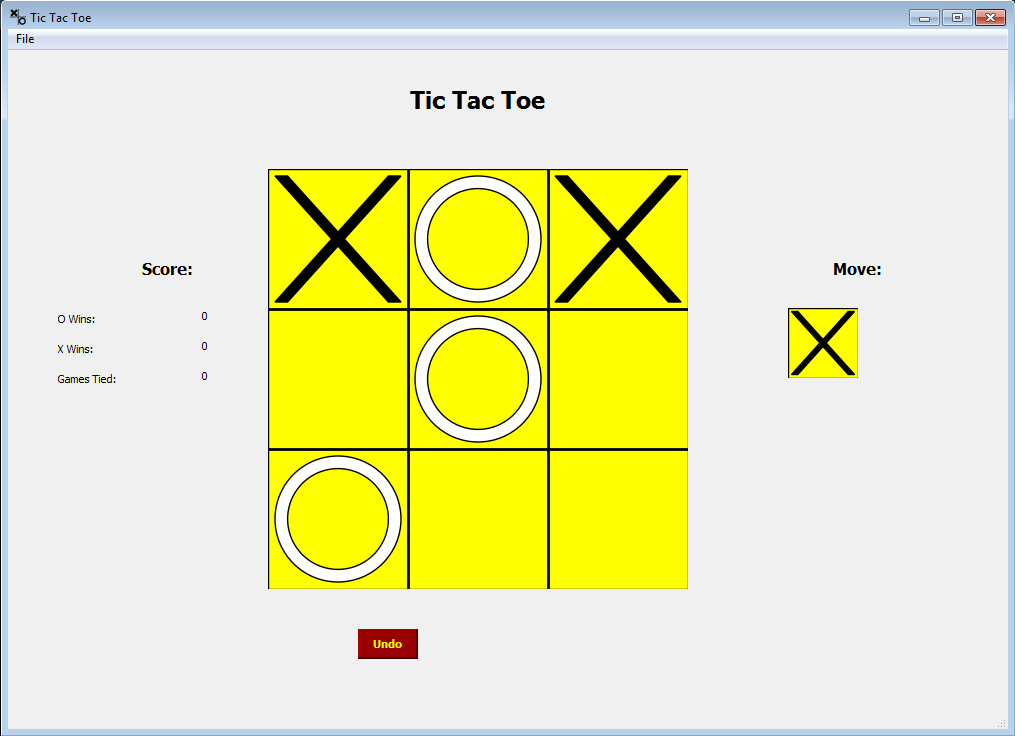
\includegraphics[width=0.8\textwidth]{TicTacToeBoard.png}
    \end{figure}
\end{frame}

\section{Results}
\begin{frame}{Conclusions}
    The dstauffman library is a fun place to learn and test different Python tricks, while making it a public repository encourages good software practices such as code documentation and unit testing, and hopefully simultaneously provides code that is useful to other people.
\end{frame}

\end{document}
